\subsection{三视图形成}

在图\ref{fig:singleprojection})所示的投影面中,可以看出同一个视图能够表示不同的物体。之所以如此,主要是因为仅用一个视图只能反映物体两方向的尺寸,而空间物体需要用长宽高三个方向的尺寸帮能够将其大小形状完整清晰地表达出来。要解决投影只能够表达物体两个尺寸方向的问题,我们需要将物体向多个投影面进行投影,通过多个投影视图来实现物体上下、左右、前后各部分的形状和大小完整表达。

\begin{figure}[htbp]
\centering
\begin{tikzpicture}
\draw[line width=0.4mm](0,0)coordinate(a1)--(0,5mm)coordinate(a2)--++(30:5mm) coordinate(a3)--++(0,5mm)coordinate(a4)--++(30:5mm) coordinate(a5)--++(0,-10mm)coordinate(a6)--cycle;
\draw[line width=0.4mm](a1)--++(150:10mm)coordinate(a7)--++(0,10mm) coordinate(a8)--++(-30:5mm)coordinate(a9)--++(0,-5mm) coordinate(a10)--(a2);
\draw[line width=0.4mm](a10)--++(30:5mm)--++(0,5mm)(a3)--++(150:5mm)(a4)--++(150:5mm)--++(30:-5mm)(a5)--++(150:10mm)--++(30:-10mm);
\draw[line width=0.4mm](a7)++(150:12mm)coordinate(b1)--++(0,5mm)coordinate(b2)--++(30:5mm) coordinate(b3)--++(0,5mm)coordinate(b4)--++(30:5mm) coordinate(b5)--++(0,-10mm)coordinate(b6)--cycle;
\begin{scope}
\clip (a8)rectangle($(a8)+(-2mm,2mm)$);
\draw(a6)--(b6);
\end{scope}
\draw[line width=0.4mm](b1)--++(150:10mm)coordinate(b7)--++(0,10mm)--++(-30:5mm)--(b2);
\draw[line width=0.4mm](b5)--++(150:10mm)--++(30:-10mm) (b4)--++(150:5mm)coordinate(b8)--++(30:-5mm)(b8)--(b3);
\draw[line width=0.4mm](b7)++(150:15mm)coordinate(c1)--++(0,5mm)coordinate(c2)--++(30:5mm) coordinate(c3)--++(0,5mm)coordinate(c4)--++(30:5mm) coordinate(c5)--++(0,-10mm)coordinate(c6)--cycle;
\draw[line width=0.4mm](c2)--++(0,5mm)coordinate(c7)--(c4);
\begin{scope}
\clip ($(b7)+(0,10mm)$) coordinate(c8)rectangle($(c8)+(-2mm,2mm)$);
\draw(b6)--(c6);
\end{scope}
\draw(a1)--(c1)(a2)--(c2)(a4)--(c4)(a5)--(c5)(a9)--(c7);
\begin{scope}
\draw($(c1)+(30:-10mm)+(0,-3mm)$)--++(0,20mm)--++(30:30mm)--++(0,-20mm)--cycle;
\end{scope}
\end{tikzpicture}
\caption{一个投影面不能确定物体在空间中的形状和位置}\label{fig:singleprojection}
\end{figure}

\begin{figure}[htbp]
\centering
\subfloat[物体在三面投影中的投影]{\label{fig:threeviewprojection}
\begin{tikzpicture}
\begin{scope}[scale=0.5]
\draw[line width=0.4mm](0,0)coordinate(a1)--(0,10mm)coordinate(a2)--++(0:10mm) coordinate(a3)--++(0,10mm)coordinate(a4)--++(0:10mm) coordinate(a5)--++(0,-20mm)coordinate(a6)--cycle;
\draw[line width=0.4mm](a1)--++(135:10mm)coordinate(a7) 
(a2)--++(135:10mm)coordinate(a8) (a3)--++(135:10mm)coordinate(a9) (a4)--++(135:10mm)coordinate(a10)(a5)--++(135:10mm)coordinate(a11);
\draw[line width=0.4mm](a7)--(a8)--(a9)--(a10)--(a11);
\draw(a1)--++(0,-15mm)coordinate(b1);
\draw[line width=0.4mm](b1)--++(135:10mm)coordinate(b2)--++(0:20mm) coordinate(b3)--++(135:-10mm)coordinate(b4)--cycle;
\draw[line width=0.4mm](b1)++(0:10mm)coordinate(b5)--++(135:10mm);
\draw(a7)--++(135:20mm)coordinate(c1);
\draw[line width=0.4mm](c1)--++(0,10mm) coordinate(c2)--++(0:10mm) coordinate(c3)--++(0,10mm) coordinate(c4)--++(0:10mm) coordinate(c5)--++(0,-20mm) coordinate(c6)--cycle;
\draw(a6)--++(0:15mm)coordinate(d1);
\draw[line width=0.4mm](d1)--++(0,20mm)coordinate(d2)--++(135:10mm) coordinate(d3)--++(0,-20mm)coordinate(d4)--cycle;
\draw[line width=0.4mm](d1)++(0,10mm)coordinate(d5)--++(135:10mm);

\draw($(b2)+(135:20mm)+(-15mm,0)$)coordinate(e1)--++(0,50mm)coordinate(e2);
\draw(e1)--++(135:-45mm)coordinate(e3);
\begin{scope}
\clip(a1)--++(135:10mm)--++(-40mm,0)--++(135:-10mm)--cycle;
\draw(e1)--++(50mm,0)coordinate(e4);
\end{scope}
\draw(e2)--++(50mm,0)coordinate(e5);
\draw(e3)--++(50mm,0)coordinate(e6);
\begin{scope}
\clip(a5)--(a11)--++(0,35mm)--++(135:-10mm)--cycle;
\draw(e4)--(e5);
\end{scope}
\begin{scope}
\clip(a6)--++(0,-35mm)--++(40mm,0)--++(0,35mm)--cycle;
\draw(e6)--(e4);
\end{scope}
\draw(e6)--++(0,50mm)coordinate(e7)--(e5);
\draw(a8)--(c2)(a9)--(c3)(a10)--(c4)(a11)--(c5)(a7)--(b2)(a3)--(b5)(a6)--(b4)(a3)--(d5)(a5)--(d2)(a11)--(d3);
\draw(e2)++(1mm,-3mm)node[below,right]{\tiny $V$ 主视图};
\draw(e3)++(1mm,2mm)node[below,right]{\tiny $H$ 俯视图};
\draw(e7)++($(135:25mm)+(0,-3mm)$)node[below,right,rotate=-45]{\tiny 左视图 $W$};
\draw[->,line width=0.3mm](e1)++(10mm,-15mm)node[left]{\tiny 左视方向}--++(10mm,0);
\draw[->,line width=0.3mm](e6)++(-15mm,-3mm)node[below,sloped]{\tiny 主视方向}--++(135:10mm);
\draw[->,line width=0.3mm](e5)++(-15mm,5mm)node[above]{\tiny 俯视方向}--++(0,-10mm);
\end{scope}
\end{tikzpicture}}
\subfloat[三个投影面的展开]{\label{fig:threeviewzhankai}
\begin{tikzpicture}
\begin{scope}[scale=0.45]
\draw(0,0)coordinate(a1)--++(0,50mm) coordinate(a2)--++(50mm,0) coordinate(a3)--++(0,-50mm) coordinate(a4)--cycle;
\draw(a1)--++(-50:50mm)coordinate(a5)--++(50mm,0) coordinate(a6)--(a4);
\draw(a3)--++(-40:50mm)coordinate(a7)--++(0,-50mm) coordinate(a8)--(a4);
\draw[line width=0.4mm](a1)++(15mm,15mm)coordinate(b1)--++(20mm,0)coordinate(b2) --++(0,20mm)coordinate(b3)--++(-10mm,0)--++(0,-10mm)--++(-10mm,0)--cycle;
\draw(b1)--++(0,-15mm)coordinate(b4)(b2)--++(0,-15mm)(b2)--++(15mm,0)coordinate(b5)(b3)--++(15mm,0);
\draw(b4)--++(-50:20mm)coordinate(c1);
\draw[line width=0.4mm](c1)--++(20mm,0)coordinate(c2)--++(-50:10mm)--++(-20mm,0)--cycle;
\draw[line width=0.4mm]($(c1)+(10mm,0)$)--++(-50:10mm);
\draw(c2)--++(-50:-20mm);
\draw(b5)--++(-40:20mm)coordinate(d1);
\draw[line width=0.4mm](d1)--++(0,20mm)coordinate(d2)--++(-40:10mm)--++(0,-20mm)--cycle;
\draw[line width=0.4mm](d1)++(0,10mm)--++(-40:10mm);
\draw(d2)--++(-40:-20mm);
\draw(a2)++(1mm,-3mm)node[below,right]{\tiny $V$ 主视图};
\draw(a5)++(1mm,2mm)node[below,right]{\tiny $H$ 俯视图};
\draw(a7)++($(-40:-25mm)+(0,-3mm)$)node[below,right,rotate=-40]{\tiny 左视图 $W$};
\draw[->,line width=0.3mm](a5)arc(-50:-80:20mm);
\draw[->,line width=0.3mm](a7)arc(-40:-10:20mm);
\end{scope}
\end{tikzpicture}}

\subfloat[展开后的三视图]{\label{fig:threeview}
\begin{tikzpicture}
\begin{scope}[scale=0.4]
\draw(0,-50mm)--(0,50mm)--++(100mm,0)--++ (0,-50mm)--++(-50mm,0)--++(0,-50mm)--cycle;
\draw(0,0)--++(50mm,0)--++(0,50mm);
\draw[line width=0.4mm](15mm,15mm)--++(20mm,0)--++(0,20mm)--++(-10mm,0) --++(0,-10mm)--++(-10mm,0)--cycle;
\draw[line width=0.4mm](70mm,15mm)--++(0,20mm)--++(10mm,0)--++(0,-20mm)--cycle;
\draw[line width=0.4mm](70mm,25mm)--++(10mm,0);
\draw[line width=0.4mm](15mm,-20mm)--++(20mm,0)--++(0,-10mm)--++(-20mm,0)--cycle;
\draw[line width=0.4mm](25mm,-20mm)--++(0,-10mm);
\draw(0,50mm)++(1mm,-3mm)node[below,right]{\tiny $V$ 主视图};
\draw(0,-50mm)++(1mm,2mm)node[below,right]{\tiny $H$ 俯视图};
\draw(100mm,50mm)++(-29mm,-4mm)node[below,right]{\tiny 左视图 $W$};
\end{scope}
\end{tikzpicture}}
\subfloat[最终三视图]{\label{fig:threeviewguilu}
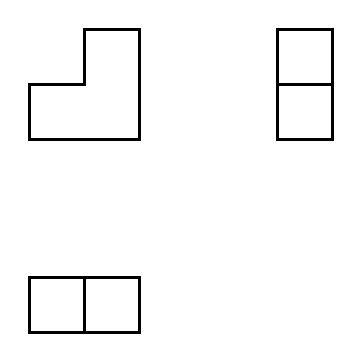
\begin{tikzpicture}
\begin{scope}[scale=0.7]
\draw[line width=0.4mm](0,0)coordinate(a1)--++ (20mm,0)coordinate(a2)--++ (0,20mm)coordinate(a3)--++ (-10mm,0)coordinate(a4)--++(0,-10mm)coordinate(a5)--++ (-10mm,0)coordinate(a6)--cycle;
\draw[line width=0.4mm](a1)++(0,-25mm)coordinate(b1)--++(0,-10mm) coordinate(b2)--++(20mm,0)coordinate(b3)--++(0,10mm) coordinate(b4)--cycle;
\draw[line width=0.4mm](b1)++(10mm,0)--++(0,-10mm);
\draw[line width=0.4mm](a2)++(25mm,0)coordinate(c1)--++(10mm,0)coordinate(c2)--++(0,20mm) coordinate(c3)--++(-10mm,0)coordinate(c4)--cycle;
\draw[line width=0.4mm](c1)++(0,10mm)--++(10mm,0);
\end{scope}
\end{tikzpicture}}
\caption{三视图的形成}
\end{figure}

 根据国家标准规定,选三个相互垂直的投影面构成图\ref{fig:threeviewprojection}所示的三投影面体系。在三视图投影体系中,正对观察者的投影面称为正平面,用$V$表示。水平放置的投影面称水平面,用$H$表示。侧立的投影面称为侧平面,用$W$表示。将物体放置于三视图投影体系中,将其由前向后投影所得的$V$面视图称为主视;将其由上向下投影所得的$H$面视图称为府视图;将物体由左向右投影所得的$W$面视图称为左视图。最后,按照国家标准,以图\ref{fig:threeviewzhankai}所示方式展开,即以$V$面视图为基准,$H$面绕$V$面与$H$面的交线所形成的$X$轴向下旋转$90\degree$;$W$面绕$V$面与$W$面的交线所形成的$Z$轴向右旋转$90\degree$,使$V$、$H$、$W$面处于同一个平面内,如图\ref{fig:threeview}所示。展开后的三视图既不需要画边框和投影轴,也不需要标视图名称,如图\ref{fig:threeviewguilu}所示。
\endinput